\begin{table}[t]
\centering
\small
\caption{One \lipi{} fact (user u02, relation \emph{home city}, answer \emph{Pune}) in its nine parallel forms, with its questions. \form{CM-R} and \form{CM-N} (likewise \form{MO-N} and \form{MO-R}) use the same words in different scripts.}
\label{tab:example}
\begin{tabular}{@{}l l >{\raggedright\arraybackslash}p{10.6cm}@{}}
\toprule
Form & Type & Memory text \\
\midrule
\form{EN} & English & Finally shifted to Pune last week, found a flat just ten minutes from the office. \\
\midrule
\form{hi-CM-R} & code-mixed, Latin & Finally last week Pune shift ho gayi, office se das minute pe flat mil gaya. \\
\form{hi-CM-N} & code-mixed, native & \adjustbox{valign=t}{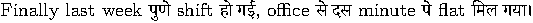
\includegraphics{indic/ex_hi_cm_nat.pdf}} \\
\form{hi-MO-N} & monolingual, native & \adjustbox{valign=t}{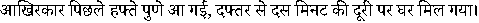
\includegraphics{indic/ex_hi_mono_nat.pdf}} \\
\form{hi-MO-R} & monolingual, Latin & aakhirkaar pichhle hafte Pune aa gayi, daftar se das minute ki doori par ghar mil gaya. \\
\midrule
\form{kn-CM-R} & code-mixed, Latin & Finally last week Pune ge shift aade, office inda hattu nimisha dooradalli flat sikkitu. \\
\form{kn-CM-N} & code-mixed, native & \adjustbox{valign=t}{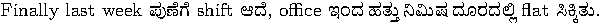
\includegraphics{indic/ex_kn_cm_nat.pdf}} \\
\form{kn-MO-N} & monolingual, native & \adjustbox{valign=t}{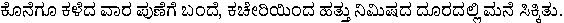
\includegraphics{indic/ex_kn_mono_nat.pdf}} \\
\form{kn-MO-R} & monolingual, Latin & konegu kaleda vaara Punege bande, kacheriyinda hattu nimishada dooradalli mane sikkitu. \\
\midrule
Question & EN & Which city do I live in now? \\
Question & hi-CM-R / hi-MO-N & \adjustbox{valign=t}{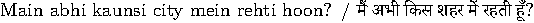
\includegraphics{indic/ex_q_hi.pdf}} \\
Question & kn-CM-R / kn-MO-N & \adjustbox{valign=t}{
\includegraphics{indic/ex_q_kn.pdf}} \\
\bottomrule
\end{tabular}
\end{table}
